%
% First comes an example EPS file -- just ignore it and
% proceed on the \documentclass line
% your LaTeX will extract the file if required
\begin{filecontents*}{example.eps}
%!PS-Adobe-3.0 EPSF-3.0
%%BoundingBox: 19 19 221 221
%%CreationDate: Mon Sep 29 1997
%%Creator: programmed by hand (JK)
%%EndComments
gsave
newpath
  20 20 moveto
  20 220 lineto
  220 220 lineto
  220 20 lineto
closepath
2 setlinewidth
gsave
  .4 setgray fill
grestore
stroke
grestore
\end{filecontents*}
%
\RequirePackage{fix-cm}
%
% \documentclass{svjour3}                     % onecolumn (standard format)
%\documentclass[smallcondensed]{svjour3}     % onecolumn (ditto)
\documentclass[smallextended]{svjour3}       % onecolumn (second format)
%\documentclass[twocolumn]{svjour3}          % twocolumn
%
\smartqed  % flush right qed marks, e.g. at end of proof
%
\usepackage{graphicx}
\usepackage[most]{tcolorbox}
\usepackage{listings}
\usepackage{xcolor}
\usepackage{subcaption}
\usepackage{tabularx}
\usepackage{booktabs}
\usepackage[colorinlistoftodos,prependcaption,textsize=tiny]{todonotes}
\usepackage{wrapfig}

\definecolor{backcolor}{rgb}{0.95,0.95,0.92}
\colorlet{punct}{red!60!black}
\definecolor{delim}{RGB}{20,105,176}
\colorlet{numb}{magenta!60!black}

\lstdefinestyle{mystyle}{
  language=Python,
  basicstyle=\ttfamily\footnotesize,
  keywordstyle=\color{delim},
  stringstyle=\color{punct},
  commentstyle=\color{numb},
  breakatwhitespace=true,
  breaklines=true,
  keepspaces=true,
  showspaces=false,
  showstringspaces=false,
  showtabs=false,
  tabsize=2,
  stepnumber=1,
  numbersep=3pt,
  captionpos=b,
  numbers=left,
  numberstyle=\tiny\color{gray},
  backgroundcolor=\color{backcolor},
  aboveskip=0pt,
  belowskip=0pt
}
\lstset{style=mystyle}

\lstset{emph={%  
    assert%
    },emphstyle={\color{delim}}%
}%

%
% \usepackage{mathptmx}      % use Times fonts if available on your TeX system
%
% insert here the call for the packages your document requires
%\usepackage{latexsym}
% etc.
%
% please place your own definitions here and don't use \def but
% \newcommand{}{}
%
% Insert the name of "your journal" with
% \journalname{myjournal}
%
\begin{document}

\title{Exploring the Role of Feedback in Machine Learning Jupyter Notebooks}

%\titlerunning{Short form of title}        % if too long for running head

\author{Arumoy Shome\and
  Lu{\`\i}s Cruz\and
  Diomidis Spinellis\and
  Arie van Deursen
}

%\authorrunning{Short form of author list} % if too long for running head

\institute{A. Shome \at
  Delft University of Technology\\
  \email{a.shome@tudelft.nl}
  \and
  L. Cruz \at
  Delft University of Technology\\
  \email{l.cruz@tudelft.nl}
  \and
  D. Spinellis \at
  Delft University of Technology\\
  \email{d.spinellis@tudelft.nl}
  \and
  A. V. Deursen \at
  Delft University of Technology\\
  \email{arie.vandeursen@tudelft.nl}
}

\date{Received: date / Accepted: date}
% The correct dates will be entered by the editor


\maketitle

\begin{abstract}

  \todo{update the numbers here}
Testing ML systems is a highly interactive process which demands a human-in-the-loop approach. In addition to writing tests for the code base, practitioners are required to analyse and interpret several visualisations using their domain expertise to validate if an ML system satisfies the required set of functional and non-functional properties. Visualisations are frequently used to qualitatively assess various parts of an ML pipeline. However, implicit knowledge gained from visualisations must be translated to explicit analytical tests that fail when there is change in any component of the ML pipeline. We conduct an empirical analysis of Jupyter notebooks to catalogue the state-of-the-art mappings between ML visualisations and assertions. We mine Github to collect 54K Jupyter Notebooks that contain assertions written in Python. We develop a novel methodology to identify 1764 notebooks which contain an assertion below a visualisation. We manually analyse the 1.7K notebooks and identify 269 visualisation-assertion pairs that are semantically related to one another. We further investigate the 269 visualisation-assertion pairs and identify three frequently occurring testing patterns. We perform an in-depth analysis of 34 visualisation-assertion pairs and find that the assertions often fail to capture all the information present in their visual counter-part. Empirical evidence obtained in this study indicates that current software testing methods fail to address the unique challenges of ML. And emphasises the need for automated tools that bridge the gap between visual assessments and analytical assertions.

\keywords{ML Testing \and SE4AI \and Visualisations \and Assertions \and Computational Notebooks}
\end{abstract}

\section{Introduction}

Machine Learning Development Lifecycle (MLDL) encompasses multifaceted series of entangled stages. Significant effort is invested in gathering and assembling the required data from diverse sources. The data then undergoes cleaning and preprocessing to ensure high quality and usability, in the subsequent stages. MLDL is dominated by the model development phase which is highly experimental and iterative. This stage involves Exploratory Data Analysis (EDA) to uncover underlying patterns, fitting the data to various models, and rigorously analyzing the results. Often, this stage may lead to additional rounds of feature engineering, where new attributes are created based on insights gained from initial models to enhance model performance. Practitioners may also engage in comparing and contrasting different models to identify the most effective approach, followed by fine-tuning selected models to optimize performance. The final model is then deployed into production where it is continuously monitored, and periodically retrained to adapt to new data or changing conditions~\cite{haakman2021ai,amershi2019software,sculley2015hidden}.

% The feedback-driven style of development in MLDL resembles principles of Agile software development and the Cross-Industry Standard Process for Data Mining (CRISP-DM). Agile methodologies emphasize continuous iteration of development and testing throughout the software lifecycle. In Agile, software is developed in incremental, rapid cycles resulting in small, incremental releases with each release building on previous functionality. Each iteration is reviewed and critiqued by the project team, which includes representatives of the project's various stakeholders. 


The MLDL is fundamentally iterative, closely resembling Agile software engineering principles which emphasize incorporating early feedback and working in small, manageable iterations.
Similarly, CRISP-DM---the dominant process model in data mining---outlines a cyclical process that evolves from understanding the business objectives and data, through data preparation, modeling, and evaluation, to deployment and monitoring. Both systems advocate for a dynamic, iterative approach that enhances adaptability and effectiveness in dealing with complex, changing systems like those encountered in ML projects.

Jupyter notebooks provide an interactive computing environment that allow users to break complex code into smaller, more manageable chunks. Each notebook is composed of a series of code cells, which can be executed independently in a Read-Eval-Print Loop (REPL) style of development. This REPL approach allows users to write a piece of code, run it, and immediately see the results thus facilitating an incremental and iterative style of software development. This modular structure of notebooks provides users the flexibility to experiment with different approaches and algorithms. Users can test hypotheses, debug issues, and make incremental changes with immediate feedback. The ability to visualize data and results inline and document the process in a narrative form further enhances their utility.

% It aligns perfectly with the feedback-driven nature of machine learning development, as it supports rapid prototyping and iterative refinement of models.

% TODO: back the TDD angle not only from scientific literature but also general methodologies used and adopted by the software engineering community (Xtreme programming, Kent Beck)

The predominant form of obtaining feedback in Jupyter notebooks is through the output of code cells. These outputs can come from three main sources in the source code--print statements, the last statement in code cells, and statements that create visualizations. Building on the principles from software engineering, we also recognize assert statements as a valuable form of feedback for writing ML code. This idea draws from prior literature in software engineering that connects test-driven development (TDD) as a form of developing software using feedback.

% TODO cite scully and breck and the data validation papers here...
% TODO: why are we doing this? how is the prior work lacking? why is this important?

In Jupyter notebooks, feedback is crucial for making important decisions throughout the machine learning development lifecycle. Practitioners rely on the output of cells to determine the appropriate data preprocessing techniques, create new features to boost model performance, and select specific hyperparameters. However, these decisions are often based on the conditions present when the model was initially created. As data, personnel, and system environments inevitably change, undocumented decisions can lead to significant technical debt. This not only prolongs debugging and troubleshooting times but also incurs additional costs and resource expenditures.

In software engineering, tests are employed to document the expected behavior of code. Failing tests indicate when these expectations are no longer met. Similarly, assertions in Jupyter notebooks can serve as documentation for the decisions made during model development. By embedding assertions, developers ensure that any deviations from expected data conditions or model performance are promptly detected, thus maintaining the integrity of the ML pipeline.

% TODO introduce our results and key findings...

% and then to tie the two things together: are assertions derived from the output of a cell? we still need to find a way to justify why we only look at assertions derived from visualisations specifically

% By analyzing the outputs and assertions in Jupyter notebooks, we aim to provide insights into the feedback mechanisms used in machine learning development, ultimately proposing strategies to improve the efficiency and robustness of this iterative process.

% Visualisations are used throughout the ml development lifecycle to test various properties of the ml system. in the early stages of the ml development lifecycle, visualisations are extensively used to make sense of the data and verify its statistical properties. during the model development phase, visualisations are used to summarise metrics, contrast different learning algorithms and iteratively fine-tune ml models. once the model is deployed in production, visualisations are used to continually monitor their performance and trigger a new training cycle once their performance drops below a certain threshold~\cite{yuan2021survey,hohman2019visual,amershi2015modeltracker,wexler2020if}.

% building ml systems is highly iterative and experimental. information gained from ml visualisations is used to make design and implementation decisions for the following steps of the ml pipeline. for instance, we may visualise the distribution of our training data and find that it is normally distributed. based on this information, we may opt for a linear regression model which assumes normality in the underlying data. however, such expectations regarding the data may be violated once the ml system is deployed in production, where the data constantly changes as a reflect of the real world~\cite{amershi2019software,sambasivan2021everyone,breck2019data,baylor2017tfx}.

% implicit expectations obtained from visualisations must therefore be translated to analytical tests that fail once our expectations regarding the ml system are no longer satisfied.

% in contrast to prior work, we approach ml testing from a new perspective. we conduct an empirical analysis of computational notebooks obtained from github, to understand the process of testing ml systems in practice. in particular, we focus on the combination of a qualitative form of testing (using visualisations) and a quantitative form of testing (using analytical assertions). the research questions along with the contributions of this paper are as follows.

% our observations indicate that formulating analytical assertions from visualisations is an emerging testing technique. however, the assertions found in this study often do not reflect the information obtained from their visual counter-part. this study finds the need for automated tools that can reduce the manual effort necessary to validate visualisations in ml systems. and help ml practitioners to formulate better analytical assertions from visualisations.

% the replication package for this study is made public on figshare\footnote{the replication package can be found at this url: https://figshare.com/s/9347228011999cba29f5}.

\section{Preliminaries}\label{sec:prelim}

This section summarises prior scientific work that has been done in ML
Testing, computational notebooks and visual analytics. The section
concludes with an overview of technical knowledge required for this
paper.

\subsection{ML Testing}\label{sec:ml-testing}

Testing ML enabled software systems poses more challenges compared to
their traditional counter part. While traditional software systems
mature through change in their codebase, ML enabled systems
additionally experience change in the training data and the machine
learning
model~\cite{sculley2015hidden,amershi2019software,sambasivan2021everyone}.
With ML being adopted into safety-critical domains that can affect
human lives, ensuring that ML systems are correct, robust to data
perturbations and not biased by race, colour or gender is of paramount
importance. Existing scientific literature on ML testing broadly
focuses on two aspects. First, on functional properties such as
correctness and robustness of the model towards unseen data. And
second, on non-functional properties such as fairness,
interpretability and
privacy~\cite{zhang2020machine,mehrabi2021survey,chen2022fairness}.

To test the correctness of ML models, several improvements over
existing test adequacy metrics have been proposed. Tools such as
\textit{DeepExplore} and \textit{DeepGauge} propose new test adequacy
metrics such as neuron coverage adapted for ML enabled software
systems~\cite{pei2017deepexplore, ma2018deepgauge,
  gerasimou2020importance}. Formal verification methods have also been
proposed that try to provide formal guarantee of robustness against
adversarial examples. Such methods however are only feasible for
statistical ML models and become computationally expensive for more
complex models such as deep neural networks~\cite{zhu2021deepmemory,
  baluta2021scalable}. Several works have been conducted on generating
and detecting adversarial inputs for ML models. Data augmentation
techniques based on fuzzing, search based software testing and
mutation testing have been proposed to generate adversarial examples
that can be used during model training to improve its
robustness~\cite{braiek2019deepevolution, gao2020fuzz, wang2021robot,
  zhang2020white}. It is however not possible to include all
variations of adversarial examples into the training data. Thus,
methods have been proposed to detect adversarial inputs during
runtime~\cite{xiao2021self, wang2020dissector, wang2019adversarial,
  berend2020cats}.

In contrast to existing scientific contributions, we conduct a
large-scale empirical analysis of Jupyter Notebooks to understand the
process of testing ML systems. Specifically, we focus on how
visualisations are used to test specific properties of ML systems. We
further investigate how frequently analytical tests are formulated
based on the information gained from the visualisations.

\subsection{Computational Notebooks and Software Engineering}\label{sec:notebooks}

Computational notebooks have been ubiquitously adopted by the machine
learning community for developing ML enabled systems. Although
originally intended to promote reproducible software, computational
notebooks are far from being reproducible due to lack of software
engineering best practices such as separation of concern, testing and
versioning~\cite{pimentel2019large,wang2020better,chattopadhyay2020wrong}.

\emph{Psallidas et al} provide an overview of the evolving landscape
of computational notebooks by analysing six million Python notebooks,
two million enterprise Data Science (DS) pipelines, source code and
metadata from over 900 releases of 12 important DS libraries. Their
findings can be used by system builders for improving DS tools and
also by DS practitioners to understand the current trends in
technologies they should focus on. \emph{Pimentel et al} mined 1.4
million notebooks from Github to conduct an empirical study on the
coding practices in computational notebooks. Based on their analysis,
the authors propose guidelines on improving reproducibility of
computational notebooks. To enable future research on computational
notebooks, \emph{Quaranta et al} mine Kaggle and present
\textit{KGTorrent}, a public dataset consisting of approximately 2.5
million Jupyter notebooks written in Python. The dataset also contains
a relational database dump of metadata regarding publicly available
notebooks on Kaggle.

Studies with human subjects have been conducted to gain a deeper
understanding of the challenges faced by ML practitioners when
developing ML models inside notebooks. The results indicate that ML
practitioners work in a highly iterative fashion, often experimenting
with multiple strategies to analyse the data or produce meaningful
visualisations~\cite{kandel2012enterprise, kery2018story,
  liu2019understanding, chattopadhyay2020wrong}. Studies have also
been conducted to understand how practitioners generate, evaluate and
manage alternative hypothesis, visual designs, methods, tools,
algorithms and data sources to arrive at the final
implementation~\cite{liu2019understanding,kandel2012enterprise}. The
findings from these studies can be used as guidelines for improving
existing notebook technologies or designing new ones.

To manage and prune multiple versions of code that accumulate over
time when developing in notebooks, \emph{Head et al} propose a code
gathering tool that allows practitioners to review and only keep the
relevant version of code. Other tools such as \textit{WrangleDoc} and
\textit{VizSmith} have also been proposed to aid ML practitioners when
working within computational notebooks~\cite{yang2021subtle,
  bavishi2021vizsmith}.

Jupyter notebooks have been widely adopted by the DS and ML
communities to develop ML
pipelines~\cite{wang2020assessing,pimentel2019large,quaranta2021kgtorrent}.
Computational notebooks provide a rich source of data in the form of
natural text, code and visualisations. Computational notebooks also
allow ML practitioners to present the knowledge gained from the
analysis in a narrative that can be shared with
others~\cite{rule2018exploration}. This study leverages the
computational narrative present within notebooks to identify
visualisations and assertions that are semantically linked to each
other.

\subsection{Visualisations and Machine Learning}\label{sec:visualisations}

As ML augment software systems in safety-critical domains, emphasis
has been put into explainability of ML models. ML models and the
underlying data is complex and multi-dimensional. To combat the
``curse of dimensionality'', visual analytics has been widely adopted
by the ML community to understand the data and the internal workings
of ML models~\cite{yuan2021survey,hohman2019visual,wexler2020if}.

Prior studies have been conducted to understand how visual analytics
techniques are currently being used in ML. \emph{Yuan et al} conduct a
systematic review of 259 papers and propose a taxonomy of visual
analytics techniques for ML. \emph{Hohman et al} conduct a survey of
visual analytics techniques for Deep Learning Models. The findings of
the study indicate that visual analytics has been widely adopted in ML
for model explanation, interpretation, debugging and improvement.

Several tools have been proposed by the visual analytics research
community to aid practitioners in understanding how their ML models
operate. \emph{Wexler et al} propose \textit{What-If}, a visual
analytics tool to explore alternative hypotheses, generate
counterfactual reasoning, investigate decision boundaries of the model
and how change in data affects the model predictions. To reduce the
cognitive load of ML practitioners during model building phase,
\emph{Amershi et al} propose \textit{ModelTracker}. Given a trained
model and a sample dataset, ModelTracker presents all the information
in traditional summary statistics along with the performance of the
model.

\textit{ESCAPE}, \textit{GAM Coach}, \textit{Angler} and
\textit{Drava} are a few other tools that have been proposed to handle
specialised use-cases such as identifying systematic errors in ML
models, generating counterfactual explanations for Generalised
Additive Models, prioritising machine translation model improvements
and relating human concepts with semantic dimensions extracted by ML
models during disentangled representation learning\cite{ahn2023escape,
  wang2023gam, robertson2023angler, wang2023drava}.

In contrast to prior work which propose dedicated visual analytics
tools, this study focuses on visualisations within computational
notebooks. We focus on visualisations produced by AI practitioners
using Python libraries (such as Matplotlib or Seaborn). Additional
context provided by surrounding code and markdown cells are used to
understand the motivation for creating the visualisation and the
information gained from it.

\section{Study Design}

\subsubsection{Motivating Example}

Sara is a data scientist who is developing a machine learning model to predict customer churn. Sara begins her project in a Jupyter notebook, which supports iterative development and immediate feedback through the execution of code cells. Her workflow is dynamic and exploratory, typical of modern machine learning practices.

Initially, Sara loads a dataset and uses basic descriptive statistics to understand its distribution. As she executes a cell that calculates and displays the mean and standard deviation of each feature, she notices unusually high variance in one of the features. This insight, derived directly from the output of the notebook cell, prompts her to apply normalization to ensure better model performance.

With data preprocessing complete, Sara proceeds to build her initial model. After setting up a logistic regression classifier, she runs a training cell that outputs the model's accuracy and loss after the first epoch. The results are disappointing, prompting her to adjust the learning rate and batch size directly in subsequent cells. Each modification is immediately followed by feedback on its impact, allowing Sara to quickly converge on the optimal settings.

Throughout this process, Sara heavily relies on the outputs of various code cells, not just for error correction but also for making strategic decisions about model architecture, such as adding layers or changing activation functions. At one point, after noticing overfitting from a cell outputting validation loss, she decides to incorporate dropout layers, which she can quickly evaluate by rerunning the training process.

Finally, Sara fine-tunes her model based on the outputs from a confusion matrix and ROC curve, identifying thresholds for classification that balance precision and recall effectively. Each decision in Sara's workflow—from preprocessing adjustments to hyperparameter tuning and model validation—is guided by the iterative feedback she receives from the outputs of her notebook's code cells.

% TODO: the jump to assertions is very drastic; motivate it using scenario that there is a bug in the system (use the data validation papers from google) and Sara needs to fix them and how assertions would have helped here to debug the issue faster! (notebook keeps running!)
Once all experimentation and model tuning are complete, and Sara is ready to deploy the model into a production environment, she adds assertions as a final step. In the dynamic, interactive environment of Jupyter notebooks, where code cells can be executed in any order, there is a risk of arriving at inconsistent states that may affect the model's performance unpredictably. Assertions act as a safeguard against these inconsistencies by verifying that the data fed into the model adheres to expected formats and distributions and that the model's performance metrics meet predetermined standards. For instance, assertions are used to ensure that no data columns have null values, that the range of input data features remains within expected bounds, and that model accuracy thresholds are consistently met regardless of the execution order of the notebook cells. This practice not only reinforces the stability and reliability of the deployed model but also provides clear, executable documentation of the critical decisions made throughout the model's development. When new team members are onboarded, these assertions allow them to quickly grasp the underlying assumptions and operational parameters of the model, ensuring ongoing robustness and performance integrity. This is crucial in maintaining the quality and reliability of the model as it transitions from a development setting to a production environment.

\subsubsection{Research Questions}

\begin{description}
  \item[RQ1.] \textbf{How is feedback from the output of code cells used when writing ML code in Jupyter notebooks?}
  \item[RQ2.] \textbf{How are assertions used to validate ML code written in Jupyter notebooks?}
  \item[RQ3.] \textbf{How are assertions used to validate visual outputs in Jupyter notebooks?}
\end{description}

\subsection{Data Collection}\label{sec:data-collect}

% TODO we need to explain why we only focus on the last statement of code cells (when visualisation code written anywhere produces an output); this is much harder to parse: we need to construct an exhaustive list of python visualisation libraries; people can use any naming convension to...

\begin{figure}
\centering
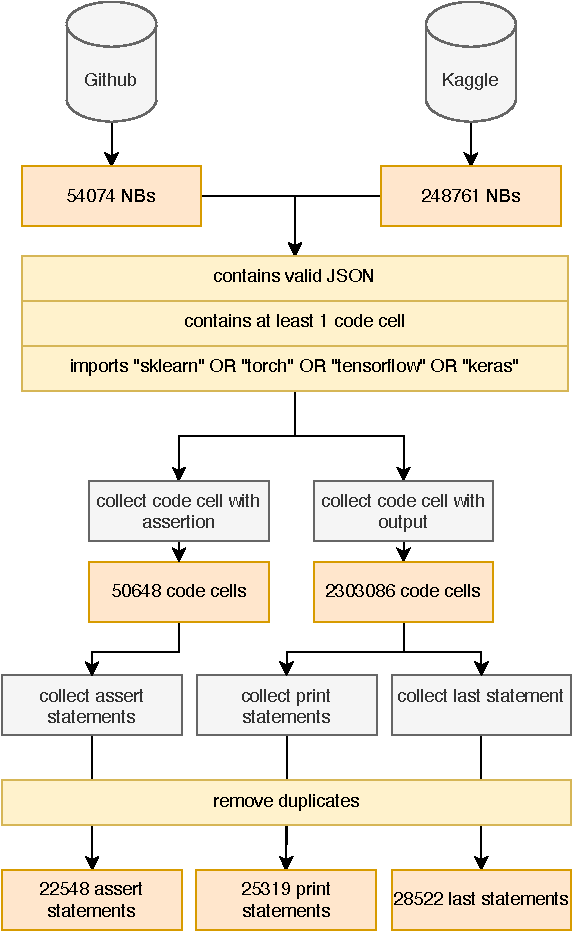
\includegraphics[width=\linewidth]{data-collection.pdf}
\label{fig:data-collection}
\caption{Overview of data collection methodology used in this study}
\end{figure}

Figure~\ref{fig:data-collection} summarises the data collection procedure used in this study. We collected Jupyter notebooks written in Python, from Kaggle and Github. 

We mined public repositories from Github to collect $49923$ Jupyter notebooks. We use the Github advanced search syntax~\footnote{https://docs.github.com/en/search-github/searching-on-github/searching-code} to isolate Jupyter Notebook that contain the keyword ``assert'' in them. The final search query is as follows: \texttt{"assert" language:"Jupyter Notebook"}.\footnote{Collected on June 22, 2023}

For Kaggle, we used a pre-existing dataset KGTorrent~\cite{quaranta2021kgtorrent} since Kaggle does not support advanced code-based search like Github. To the best of our knowledge, KGTorrent this is the largest dataset of Python Jupyter notebooks obtained from Kaggle consisting of $248763$ notebooks.

Therefore, we start with 283GB of data comprising of $298686$ Python Jupyter notebooks.

We check the validity of the underlying JSON structure in each notebook using the nbformat tool ~\footnote{https://nbformat.readthedocs.io/en/latest/}. Since the focus of this study is on the analysis of Python code, we only include notebooks that contain at least one code cell. Finally, to focus on Python code written specifically for ML projects, we only include notebooks that import popular ML libraries~\footnote{These libraries are derived from white literature---https://www.coursera.org/articles/python-machine-learning-library, https://www.geeksforgeeks.org/best-python-libraries-for-machine-learning, https://www.datacamp.com/blog/top-python-libraries-for-data-science, https://www.kdnuggets.com/2020/11/top-python-libraries-data-science-data-visualization-machine-learning.html, https://lp.jetbrains.com/python-developers-survey-2022}.

For explicit feedback using assertions, we programmatically analyse the JSON structure of the notebooks to isolate code cells. We collect Python assert statements from the code cells by constructing and subsequently parsing the Abstract Syntax Tree (AST) of the source code present in each cell.

\todo{TODO: justify why we didn't collect failures (strerr); that is more debugging? not the focus of this paper?}
Similarly, for implicit feedback, we first isolate code cells that produce an output. The output of a cell may either be from a ``print'' statement or the last statement of the cell. We collect both of them using the AST of the cell.

Finally, we remove duplicate data points (asserts, prints and last statements) resulting in a final data set of $22548$ assertions, $25319$ print statements and $28522$ last statements.

\subsection{Case Studies}

\todo{TODO: might need a visual aid here}

We allocated a fixed time resource of 100 hours to conduct the case study analysis of all candidates (assertions and cell outputs). To surface interesting candidates for the case studies, we apply NLP techniques as described below.

\todo{TODO: point out the poor quality of notebooks out there (we have citations for this); and the resulting noise in the assertions/outputs. Thats why we need to apply these techniques to surface unique and interesting candidates!}

The assertions and cell outputs are first tokenised---special characters and alpha-numeric words shorter than two characters are removed. Two stop words namely ``assert'' and ``print'' are removed since they appear in all assertions and print statements respectively. The term frequency (TF) for all tokens is calculated and then normalised using their inter-document frequency (IDF) such that tokens that appear less frequently are assigned a higher value.

We apply stratified random sampling to identify the candidates for the case study analysis. The sub-groups are created by adding TF-IDF of the tokens in each candidate to produce an aggregate value. The candidates are then divided into quartiles based on the aggregate value. A candidate is randomly drawn from each bin and analysed as an in-depth case study. The analysis is stopped when the time resource is exhausted.

During each case study, we analyse the code of the candidate to understand its purpose. Additionally, we analyse the entire code cell, the previous cell, next cell and the notebook's purpose to bring in rich context.

\section{Results}

\subsection{(RQ1) How is feedback from the output of code cells used when writing ML code in Jupyter notebooks?}

\subsubsection{Data distribution check ($N = 7$)}
% (O2, O4, O9, O14, O20, O25, O48)

% TODO: we refer to these as outputs but they are actually the python statements that produce the outputs...do we need better terminology here? To me this is especially confusing because in the figure below we are actually showing the output, not the python statement (which makes sense, its more interesting to show the actual visualisation in these cases rather than the code).
\begin{table}
\centering
\caption{Examples of cell outputs used to verify distribution of data.}
\begin{tabular}{@{}m{0.05\textwidth} m{0.4\textwidth} m{0.4\textwidth}@{}}
\toprule
\emph{\textbf{Key}}&
\emph{\textbf{Code}}&
\emph{\textbf{Visual Output}}\\
\midrule

O2&
\lstinline[]$_ = sns.catplot(x='category_id', y='likes', data=train, height=5, aspect=1.5)$&
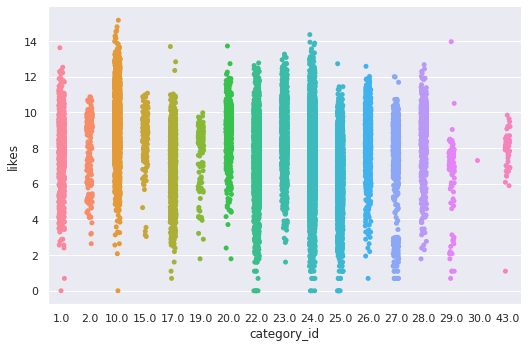
\includegraphics[width=\linewidth]{distribution-check-catplot.png}\\

O9&
\lstinline[]$sns.kdeplot(data=data.loc[ data['Survived'] == 0].Age, label='Died', shade=True)$&
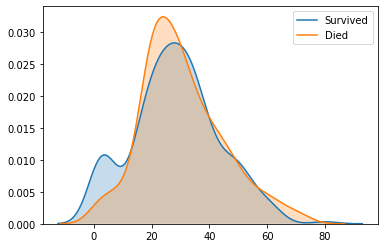
\includegraphics[width=\linewidth]{distribution-check-kdeplot.png}\\

O14&
\lstinline[]$pd.pivot_table(train, index='Survived', values=['Age', 'SibSp', 'Parch', 'Fare'])$&
\\

O25&
\lstinline[]$sns.countplot(house_pred['OverallQual'])$&
\\

O48&
\lstinline[]$x_train.describe()$&
\\

\bottomrule
\end{tabular}
\label{tab:distribution-check}
\end{table}

Table~\ref{tab:distribution-check} shows examples of outputs used to check the distribution of the data. In output \emph{O2} the distribution of feature \texttt{Age} is checked against the two labels (\texttt{Survived} and \texttt{Died}) of the target feature. Output \emph{O9} presents another example where the distribution of a continuous feature \texttt{likes} is checked with-respect-to all the values of another categorical feature \texttt{category\_id}. Output \emph{O14} produces a pandas dataframe which is used to check the mean value of the features \texttt{Age}, \texttt{SibSp}, \texttt{Parch} and \texttt{Fare} against each label in the target feature \texttt{Survived}. Output \emph{O48} produces a pandas dataframe with the descriptive statistics of all features in the training data. The statement is written immediately after normalising the features in the training data. Hence, the user manually verifies if the normalisation was successful by looking at the mean and standard deviation of the features in the output. Similarly, \emph{O25} is written after discretizing a continuous feature \texttt{OverallQual} using binning. 

% TODO: this is probably implications/discussions material?
Understanding the distribution of data is crucial for making informed decisions about necessary transformation steps in data analysis. For instance, visualizations can efficiently determine if scaling, normalizing, or handling outliers is needed. During the exploratory data analysis (EDA) phase, visualizations and pandas dataframes are commonly used to assess specific columns' distribution, helping identify features related to the target variable and informing feature inclusion in model training. Additionally, descriptive statistics are used post-transformation to verify the effectiveness of steps like data normalization, ensuring data conforms to the expected format for further analysis.

\subsubsection{Data relationship check ($N = 2$)}
% (O6, O10)

\begin{table}
  \centering
  \caption{Cell outputs used to verify linear relationship between features in the data.}
  \begin{tabular}{@{}m{0.05\textwidth} m{0.4\textwidth} m{0.4\textwidth}@{}}
    \toprule
    \emph{\textbf{Key}}&
    \emph{\textbf{Code}}&
    \emph{\textbf{Visual Output}}\\
    \midrule

    O6&
    \lstinline[]$b = sns.relplot(x='SIZE', y='Cash', hue='CLARITY', alpha=0.9, palette='muted', height=8, data=raw_data)$&
    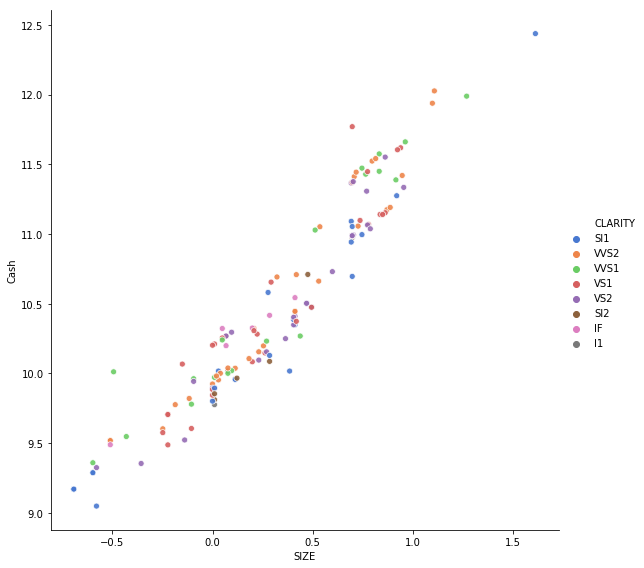
\includegraphics[width=\linewidth]{linear-relation-check-lineplot.png}\\

    O10&
    \lstinline[]$sns.regplot(x='X4 number of convenience stores', y='Y house price of unit area', data=data)$&
    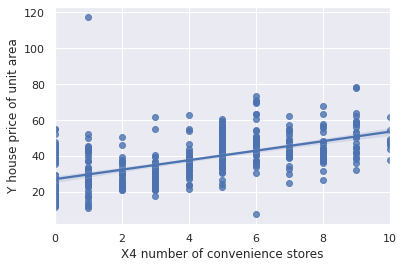
\includegraphics[width=\linewidth]{linear-relation-check-regplot.png}\\
    \bottomrule
  \end{tabular}
\label{tab:linear-relation-check}
\end{table}

Table~\ref{tab:linear-relation-check} illustrates two outputs found in this study for identifying linear relationships amongst features in the data. In output \emph{O6}, the practitioner assesses the linearity between the features \texttt{Cash} and \texttt{SIZE}. Output \emph{O10} depicts the visualization of the feature \texttt{X4} alongside the target variable \texttt{Y}, accompanied by a fitted linear regression model.

Linear machine learning models achieve optimal performance when the target variable can be expressed as a linear combination of the input features. However, features within a dataset that exhibit a linear relationship are considered redundant as they convey the same information to the model during training. Consequently, the feature engineering stage often involves removing such features to create a more efficient training dataset~\ref{shome2022data}.

\subsubsection{Resource check ($N = 7$)}\label{sec:implicit-resource-check}
% (P71, P86, O64, O66, P68, P82, P107)

\begin{table}
\centering
\caption{Examples of cell outputs used to verify if different types of resources are available on the system where the notebook is being executed.}
\begin{tabular}{@{}m{0.05\textwidth} m{0.8\textwidth}@{}}
\toprule
\emph{\textbf{Key}}&
\emph{\textbf{Code}}\\
\midrule

P68&
\lstinline[]$print('GPU is available')$\\

P71&
\lstinline[]$print('Hub version: ', hub.__version__)$\\

P82&
\lstinline[]$print('Running on TPU ', tpu.master())$\\

P86&
\lstinline[]$print('Cuda is available')$\\

P107&
\lstinline[]$print('Model loaded')$\\

O64&
\lstinline[]$full_table.head(-5)$\\

O66&
\lstinline[]$prostate_cancer_df.shape$\\
\bottomrule
\end{tabular}
\label{tab:resource-check}
\end{table}

% NOTE: O107 is a print statement which is execute even if the prior statement that loads the model fails...
Table~\ref{tab:resource-check} presents case studies where the output is used to verify availability of resources on the system in which the notebook is being executed. Outputs \emph{P68}, \emph{P82} and \emph{P86} check for the availability of compute resources, such as a GPU or a TPU. This study also finds outputs used to verify that a dataset or a pre-trained model has been successfully loaded into memory. For example, Output \emph{P107} is written after loading a pre-trained model is loaded into memory. Output \emph{O64} generates a pandas dataframe with the last five rows of the data while \emph{O66} shows the shape of the data. These statements are written directly after loading the data from the file system to manually verify that the data was loaded without errors. Additionally, output \emph{P71} is used to ensure that a certain version of an external library is present on the system.

The print statement P71 highlights the lack of proper software engineering best practices within Jupyter notebooks. This shortcoming in computational notebooks has been identified by prior studies~\cite{quaranta2021kgtorrent, pimentel2019large-scale}. In this case study, managing dependencies through external tools is recommended. Python's built-in \emph{requirements.txt}~\footnote{https://pip.pypa.io/en/stable/reference/requirements-file-format/} file allows specifying dependencies and versions. Alternatively, external programs like \emph{pipenv}~\footnote{https://pipenv.pypa.io/en/latest/} and \emph{poetry}~\footnote{https://python-poetry.org/} use lockfiles to ensure specific version control, guaranteeing reproducibility across different systems. 

\subsubsection{Execution time check ($N = 1$)}
% (P66)

\begin{table}
  \centering
  \caption{Print statement used to check the total execution time of training and cross-validating an ML model.}
  \begin{tabular}{@{}m{0.05\textwidth} m{0.8\textwidth}@{}}
    \toprule
    \emph{\textbf{Key}}&
    \emph{\textbf{Code}}\\
    \midrule

    P66&
    \lstinline[]$print('Total Run Time:')$\\
  \end{tabular}
  \label{tab:exec-time}
\end{table}

Table~\ref{tab:exec-time} presents print statement \emph{P66} which prints the total execution time of a code cell which trains an ML model with various hyper-parameter configurations using a grid-search. \emph{P66} is also used in other code cells in the notebook that train other ML models.

While training multiple machine learning models for a single task is common, choosing the best model considers not only its performance but also its training speed. Faster training times are more cost-effective for iterative tasks and promote sustainability in the long run~\cite{CITEME}.

\subsubsection{Missing value check ($N = 3$)}
% (O12, O36, P74)

\begin{table}
\centering
\caption{Examples of cell outputs used to check for missing data.}
\begin{tabular}{@{}m{0.05\textwidth} m{0.4\textwidth} m{0.4\textwidth}@{}}
\toprule
\emph{\textbf{Key}}&
\emph{\textbf{Code}}&
\emph{\textbf{Visual Output}}\\
\midrule

P74&
\lstinline[]$print(train_df.isnull().sum())$&
\\


O12&
\lstinline[]$sns.heatmap(test_df.isnull(), yticklabels=False, cbar=False, cmap='viridis')$&
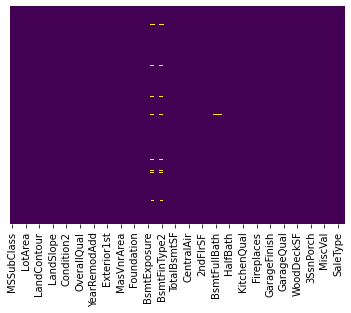
\includegraphics[width=\linewidth]{missing-value-check.png}\\

O36&
\lstinline[]$test.isna().sum().unique()$&
\\
\bottomrule
\end{tabular}
\label{tab:missing-value}
\end{table}

Table~\ref{tab:missing-value} presents all case studies where cell outputs were used to check for missing data. While \emph{P74} and \emph{O36} perform this check in code, \emph{O12} presents a visual representation of missing data using a heatmap.

Checking for missing values is a critical step in the preprocessing phase of a machine learning project because it significantly influences the quality and performance of the model. Missing data can lead to biased or incorrect conclusions if not handled properly, potentially skewing the model's performance by training on incomplete or non-representative samples~\cite{shome2022data}. Many machine learning algorithms, including those that involve matrix multiplication operations such as linear regression and neural networks, demand complete numerical datasets to perform calculations. Missing values interrupt these calculations, leading to errors or the inability to execute algorithms entirely.

\subsubsection{Model performance check ($N = 33$)}
% (O3, O50, O52, O57, O74, P3, P6, P8--12, P16--19, P23, P24, P28, P30, P34, P42, P47, P48, P50, P51, P54, P55, P57, P58, P61, P78, P93)

\begin{table}
\centering
\caption{Various cell outputs used to check the performance of an ML model after training.}
\begin{tabular}{@{}m{0.05\textwidth} m{0.4\textwidth} m{0.4\textwidth}@{}}
\toprule
\emph{\textbf{Key}}&
\emph{\textbf{Code}}&
\emph{\textbf{Visual Output}}\\
\midrule

P3&
\lstinline[]$print('The mean accuracy with 10 fold cross validation is: %s ' % round(scores * 100, 2), '%')$&
\\

P6&
\lstinline[]$print('RMSE:', np.sqrt(metrics.mean_squared_error(y_test, pred)))$&
\\

P18&
\lstinline[]$print('The Accuracy is:', accuracy_score(y_test, y_pred))$&
\\

P50&
\lstinline[]$print('Classification Report: SVM (validation data)')$&
\\

P54&
\lstinline[]$print('Intercept value:', lm.intercept_)$&
\\

O3&
\lstinline[]$skplt.metrics. plot_confusion_matrix(Y_val, Vote.predict(X_val), normalize=True, figsize=(10, 10))$&
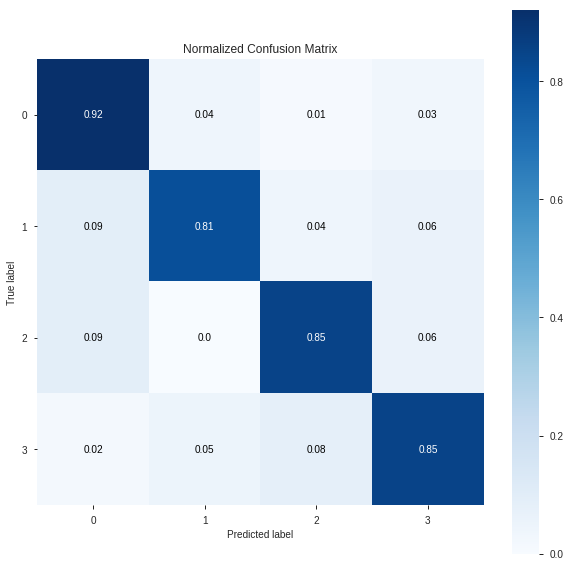
\includegraphics[width=\linewidth]{model-perf-confusion-matrix.png}\\

O52&
\lstinline[]$spot_check_recs(classifier, 910)$&
\\
\bottomrule
\end{tabular}
\label{tab:model-perf}
\end{table}

Table~\ref{tab:model-perf} presents a few examples of cell outputs used to check the performance of a trained ML model. Besides the \emph{accuracy} of the model (\emph{P3} and \emph{P18}), we also see checks for the \emph{Root Mean Square Error (RMSE)} (\emph{P6}) and the use of the classification report (\emph{P50}) provided by scikit-learn~\footnote{https://scikit-learn.org/stable/modules/generated/sklearn.metrics.classification\_report.html} which reports the \emph{accuracy}, \emph{precision}, \emph{recall} and \emph{f1 score} for all labels present in the target feature.

% TODO: this feels hallucinated; revisit
Print statement \emph{P54} prints the intercepts of a linear regression model. Checking the intercept of a linear regression model is essential for understanding the baseline prediction when all predictors are zero, interpreting the model, identifying potential data biases or missing variables, assessing model validity, and comparing baseline predictions across different models. This insight is critical for accurate model interpretation and effective decision-making in practical applications.

Output \emph{O3} shows a heatmap used to visualise the confusion matrix of a multi-label classification task. The values are normalised using the actual number of examples of each class which makes the comparisons of the values across the classes possible.

Output \emph{O52} shows a function implemented by the practitioners to manually evaluate an image classification model on a random sample of input images. The function \texttt{spot\_check\_recs} displays the input image along with the prediction of the model which the practitioner uses to spot-check the performance of the model.

During the model development phase, the performance of an ML model is often printed to facilitate comparisons against other models or variations. Throughout this continuous experimentation phase, authors may adjust model parameters or modify the data by engineering new features. The model is then re-trained to check if these changes lead to performance improvements.

\subsubsection{Neural network architecture ($N = 1$)}
% (P92)

\begin{table}
  \centering
  \caption{Print the architecture of a neural network.}
  \begin{tabular}{@{}m{0.05\textwidth} m{0.8\textwidth}@{}}
    \toprule
    \emph{\textbf{Key}}&
    \emph{\textbf{Code}}\\
    \midrule
    P92&
    \lstinline[]$print(MyNetwork)$\\
    \bottomrule
  \end{tabular}
  \label{tab:network-architecture}
\end{table}

Table~\ref{tab:network-architecture} shows print statement \emph{P92} which shows the architecture of a neural network.

Printing the structure of a neural network serves crucial purposes such as verifying the correct implementation of the architecture, aiding in debugging by ensuring layer compatibility, and providing a clear, human-readable format for documentation and educational insights. It helps in verifying configurations like layer dimensions and operations before initiating computationally intensive training, ensuring the model is set up efficiently for the intended tasks. This practice is fundamental for maintaining accuracy, facilitating collaboration, and enhancing the reproducibility of the model.

\subsubsection{Shape check ($N = 3$)}
% (P4, P32, P117)

\begin{table}
  \centering
  \caption{Example of outputs used to check the shape of the data.}
  \begin{tabular}{@{}m{0.05\textwidth} m{0.8\textwidth}@{}}
    \toprule
    \emph{\textbf{Key}} & \emph{\textbf{Code}}\\
    \midrule
    P4 &
    \lstinline[]$print('no.of examples in test data : ', len(test_data))$\\

    P32 &
    \lstinline[]$print('Training set shape : ', x_train.shape)$\\

    P117&
    \lstinline[]$print('Y_train.shape: ', Y_train.shape)$\\
    \bottomrule
  \end{tabular}
  \label{tab:shape-check}
\end{table}

Table~\ref{tab:shape-check} shows print statements discovered in this study which check the shape of the data. \emph{P4} prints the number of rows or examples in the test set. \emph{P32} and \emph{117} prints the number of rows and columns (or features) in the training and test data respectively.

Ensuring that data dimensions align with expectations is important particularly following data pre-processing or transformation steps. Primarily, the number of features in the training set must match those in the testing set. This alignment is crucial because statistical machine learning models are trained on specific data dimensions and expect the same dimensional structure during inference to perform accurately. Similarly, in neural network architectures, the configuration of input layers depends directly on the shape of the training data, dictating the number of input neurons needed. Furthermore, the correspondence between the number of test examples and their respective labels is essential for accurately computing performance metrics, such as accuracy.

Such checks are indicative of the meticulous attention to detail necessary in the model training and validation process, underscoring the importance of shape validation in achieving reliable machine learning outcomes.

\subsubsection{Type check ($N = 2$)}
% (O71, P43)

% TODO: the narrative is not as strong here; it would help to also show the actual output as well? For instance, in P43 by itself doesn't make that much sense, the output however shows that all features in the dataset are floats which is a pre-requisite for ML training data
\begin{table}
  \centering
  \caption{Outputs used to check the data type of features in the data.}
  \begin{tabular}{@{}m{0.05\textwidth} m{0.8\textwidth}@{}}
    \toprule
    \emph{\textbf{Key}} &
    \emph{\textbf{Code}}\\

    P43&
    \lstinline[]$print('data type:', images.dtype)$\\

    O71&
    \lstinline[]$type(Y)$\\
    \bottomrule
  \end{tabular}
  \label{tab:type-check}
\end{table}

% TODO: for O71, the output shows its a ndarray; without showing this to the reader we cannot make a strong narrative around these type checks
Table~\ref{tab:type-check} illustrates outputs of cells found in our analysis, where checks are employed to verify the data types of the features in the dataset. Print statement \emph{P43} is written prior to training a neural network. The output validates that all features in the training data are numerical. Similarly, output \emph{O71} shows the data type of the target column.

Type checks are crucial not only for confirming the current state of the data but also for determining the specific transformations required to make the data suitable for subsequent modelling steps. Ensuring data types align with model requirements is a fundamental step in the exploratory data analysis (EDA) phase of developing machine learning models. Since all machine learning algorithms perform mathematical operations, such as matrix multiplications, they require the input data to be entirely numerical to avoid computational errors. The process of checking data types helps in identifying the necessary pre-processing or transformation steps to convert the data into a form that is compatible with these models. For example, while numerical features often require normalisation to bring them within a specific scale, categorical features must be converted into a numerical format through methods like one-hot encoding to ensure they can be effectively integrated into the model.

\subsubsection{Spot checks ($N = 5$)}
% (O56, O60, P64, P67, P114)

\begin{table}
  \centering
  \caption{Example of outputs used to perform spot checks.}
  \begin{tabular}{@{}m{0.05\textwidth} m{0.8\textwidth}@{}}
    \toprule
    \emph{\textbf{Key}}&
    \emph{\textbf{Code}}\\
    \midrule

    O60 &
    \lstinline[]$X_pca.head()$\\

    P64 &
    \lstinline[]$print(np.max(cur[:, :, 1]))$\\

    P114 &
    \lstinline[]$print(onehot_encoded)$\\
    \bottomrule
  \end{tabular}
  \label{tab:spot-check}
\end{table}

Table~\ref{tab:spot-check} presents outputs which were used to perform spot checks at various stages of the ML development cycle. In \emph{O60}, the practitioner verifies that the number of features in the data matches expectations after apply Principal Component Analysis (PCA). \emph{P64} demonstrates another case which is particularly relevant in image processing contexts. The maximum value in the second channel of a 3D numpy array is extracted and verified, ensuring that the data manipulation retains its expected properties. Lastly, \emph{P114} assesses the correctness of one-hot encoding, a fundamental preprocessing step for categorical data, ensuring that the transformation has been executed correctly.

Performing value or spot checks can be an essential practice for ensuring data integrity and model accuracy at various stages of development. These checks are crucial for verifying that operations such as data transformations, model predictions, and feature engineering are functioning as expected. Each of these checks not only validates individual transformations or predictions but also reinforces the overall reliability and robustness of the machine learning models being developed.

% The check in P67 involves a manual verification of the output of an activation function in a neural network, which is essential for confirming the functional efficacy of neural components in model training. 

\subsubsection{Model training ($N = 4$)}
% (O8, O31, O42, P77)

\begin{table}
  \centering
  \caption{Example of outputs used to monitor model training.}
  \begin{tabular}{@{}m{0.05\textwidth} m{0.8\textwidth}@{}}
    \toprule
    \emph{\textbf{Key}}&
    \emph{\textbf{Code}}\\
    \midrule

    O8 &
    \lstinline[]$autoencoder.fit(x=X_train, y=X_train, epochs=15, validation_data=[X_test, X_test], callbacks=[keras_utils.TqdmProgressCallback()], verbose=0)$\\

    O31 &
    \lstinline[]$adaBoost.fit(X_train, y_train)$\\

    O42&
    \lstinline[]$m_r.best_params_$\\
    \bottomrule
  \end{tabular}
  \label{tab:model-training}
\end{table}

During training it is common practice to monitor progress periodically, as illustrated by outputs \emph{O8} in Table~\ref{tab:model-training}, where the training loss and accuracy are printed to give real-time feedback on the model's learning efficacy. This feedback allows for adjustments in training parameters or early stopping to prevent overfitting. For instance, in output O8, the autoencoder is trained using a custom callback from \texttt{keras\_utils} to provide a progress update without cluttering the output stream, which is particularly useful in lengthy training sessions. In contrast, output \emph{O31} represents a crucial validation step where the \texttt{adaBoost} model is fitted to the training data to ensure it adheres to the expected data patterns without errors, a typical task in the model experimentation phase where various models are assessed for their suitability. Output \emph{O42} checks for the best parameters found through tuning methods, highlighting the importance of parameter optimisation in achieving optimal model performance.

Each of these outputs underscores different facets of the model training phase, from initialization and real-time monitoring to validation and finalization, illustrating the layered complexity of developing predictive models.

\subsection{(RQ2) How are assertions used to validate ML code written in Jupyter notebooks?}

% TODO: bring in the notion of pre and post condition checks (the wikipedia page on assertions is very interesting: https://en.wikipedia.org/wiki/Assertion_(software_development)); specifically the part on run-time assertions

\subsubsection{Batch size check ($N = 3$)}
% (A21, A28, A70)

\begin{table}
  \centering
  \caption{Assertions used to validate the batch size of input data.}
  \begin{tabular}{@{}m{0.05\textwidth} m{0.8\textwidth}@{}}
    \toprule
    \emph{\textbf{Key}}&
    \emph{\textbf{Code}}\\
    \midrule

    A21 &
    \lstinline[]$assert x.size(0) % batch_size == 0, f'the first dimension of input tensor ({x.size(0)}) should be divisible by batch_size ({batch_size})'$\\

    A28 &
    \lstinline[]$assert image_size % patch_size_small == 0, 'Image dimensions must be divisible by the patch size.'$\\

    A70 &
    \lstinline[]$assert n_img > batch_size$\\
    \bottomrule
  \end{tabular}
  \label{tab:batch-size}
\end{table}

Table~\ref{tab:batch-size} shows the assertions found in this study that validate the batch size. \emph{A21} ensure that the batch size divides evenly into the training dataset size, thereby confirming that every training epoch processes full batches without leftover data. Similarly, \emph{A28} checks that image dimensions are suitably divisible by the patch size, which is essential for certain types of convolutional networks. \emph{A70} is another critical check which confirms that the number of images is greater than the batch size, which is necessary to commence batch processing.

In the context of neural network training, the practice of using batch processing is a key strategy to enhance computational efficiency and hardware utilization, particularly GPU cores. Batching allows for a more stable and smoother learning curve as the model's weights are updated not for each individual example, but rather based on the average gradient of a batch. This technique not only optimizes learning but also enhances the model's generalizability due to more robust gradient estimations. Given these benefits, it becomes crucial to ensure that the batch size is appropriately set to match the hardware's capacity, avoiding memory overflow issues that can halt training. These assertions are strategically placed to prevent common errors that could undermine training efficiency and model performance, thereby safeguarding the training process from potential disruptions due to misconfigured batch sizes.

\subsubsection{Data leakage check ($N = 1$)}
% (A33)

\begin{table}
  \centering
  \caption{Assert used to prevent data leakage.}
  \begin{tabular}{@{}m{0.05\textwidth} m{0.8\textwidth}@{}}
    \toprule
    \emph{\textbf{Key}}&
    \emph{\textbf{Code}}\\
    \midrule

    A33&
    \lstinline[]$assert len(set( tr_df.PetID.unique()).intersection(valid_df.PetID.unique())) == 0$\\
    \bottomrule
  \end{tabular}
  \label{tab:data-leakage}
\end{table}

Assertion \emph{A33} in Table~\ref{tab:data-leakage} ensures that there are no overlapping \texttt{PetID} values between the training set \texttt{tr\_df} and the validation set \texttt{valid\_df}, thereby preventing any possibility of data leakage.

Ensuring the absence of data leakage between training and validation datasets is a fundamental best practice in machine learning to prevent models from overfitting. Overfitting occurs when a model is excessively complex, learning not only the underlying patterns but also the noise in the training data, which can degrade its performance on unseen data. To guarantee that the model can generalize effectively to new examples, it's crucial to verify that the training and validation sets are completely distinct with no shared examples. By strictly separating these datasets, the validation phase serves its purpose of providing an unbiased evaluation of the model's ability to generalize---to data similar to, but not identical to that which it was trained on---thus maintaining the integrity and validity of the evaluation metrics derived during model testing.

\subsubsection{Existence check ($N = 8$)}
% NOTE: this is a combination of missing-value-check and existence-check
% (A23, A42, A43, A50, A51, A63, A79, A86)

\begin{table}
  \centering
  \caption{Assertions used to perform existence checks.}
  \begin{tabular}{@{}m{0.05\textwidth} m{0.8\textwidth}@{}}
    \toprule
    \emph{\textbf{Key}}&
    \emph{\textbf{Code}}\\
    \midrule

    A23 &
    \lstinline[]$assert np.all(orders.groupby('user_id') .days_since_prior_order.tail(1).notnull())$\\

    A42 &
    \lstinline[]$assert not lab_s.isnull().values.any()$\\

    A43 &
    \lstinline[]$assert len(data) != 0, 'cannot divide by zero'$\\

    A50 &
    \lstinline[]$assert not np.any(np.isnan(X))$\\

    A51 &
    \lstinline[]$assert data.target.notnull().all()$\\

    A63 &
    \lstinline[]$assert X.isnull().sum().sum() == 0$\\

    A79 &
    \lstinline[]$assert not processed_data_df.isna().any().any()$\\

    A86 &
    \lstinline[]$assert p0 in poi_info.index$\\
    \bottomrule
  \end{tabular}
  \label{tab:existence-check}
\end{table}

Assertions \emph{A23} and \emph{A42} in Table~\ref{tab:existence-check} ensure that specific data columns do not contain any missing entries, which could compromise the reliability of subsequent analyses. Assertion \emph{A43} guards against operations on empty datasets, which are a potential risk after filtering or merging data processes. Assertions \emph{A50}, \emph{A51} and \emph{A63} rigorously confirm that the datasets are entirely free from \texttt{NaN} values, thus preserving the integrity of the dataset for reliable model training. Assertions \emph{A79} and \emph{A86} ensure that no unexpected missing values are introduced and that all expected indices are present in the dataset respectively.

Existence checks are a fundamental component of data preprocessing in ML, serving multiple critical purposes to ensure data integrity before analysis and modeling. These checks primarily focus on verifying the presence of necessary columns and the absence of missing values within those columns. Such validations are especially crucial after data preprocessing steps, where transformations might inadvertently introduce null values. These checks are also crucial for maintaining the accuracy and efficiency of data handling processes, ensuring that the datasets are ready for robust machine learning applications.

\subsubsection{Mathematical property checks ($N = 4$)}
% (A3, A25, A56, A64)

\begin{table}
  \centering
  \caption{Assertions used to validate mathematical properties of neural networks.}
  \begin{tabular}{@{}m{0.05\textwidth} m{0.8\textwidth}@{}}
    \toprule
    \emph{\textbf{Key}}&
    \emph{\textbf{Code}}\\
    \midrule

    A3 &
    \lstinline[]$assert (xH - wH) % self.stride == 0$\\

    A25 &
    \lstinline[]$assert test_output.std() < 0.15, "Don't use batchnorm here"$\\

    A56 &
    \lstinline[]$assert np.allclose(e_v_states[:, -1], np.ones_like(e_v_states[:, -1]))$\\

    A64 &
    \lstinline[]$assert np.allclose(T, T.T)$\\
    \bottomrule
  \end{tabular}
  \label{tab:maths-check}
\end{table}

Assertion \emph{A3} in Table~\ref{tab:maths-check} checks that the dimension differences between height of input and the filter, when divided by the stride, result in an integer, ensuring that convolution operations are dimensionally consistent. \emph{A25} monitors the standard deviation of outputs to decide the appropriateness of using batch normalisation, thus guiding the model optimization process based on statistical behavior. \emph{A56} verifies the uniformity of certain computations, essential for maintaining consistency in state or parameter arrays over iterations. Similarly \emph{A64} checks for the symmetry of a matrix, a crucial property in many algorithms, particularly those involving covariance matrices and distance calculations. 

When working with neural networks and other statistical models, it is imperative to ensure that mathematical properties are preserved throughout operations involving arrays and matrices. This rigor is captured through the assertions in Table~\ref{tab:maths-check} tha validate these properties after matrix manipulations. These assertions are not just precautionary but are vital for confirming that the underpinnings of ML algorithms align with expected mathematical principles, thereby ensuring the robustness and reliability of model computations and outcomes.

\subsubsection{Model performance check ($N = 11$)}
% (A7, A15, A19, A22, A24, A26, A38, A54, A58, A59, A72)

\begin{table}
  \centering
  \begin{tabular}{@{}m{0.05\textwidth} m{0.8\textwidth}@{}}
    \toprule
    \emph{\textbf{Key}}&
    \emph{\textbf{Code}}\\
    \midrule

    A7 &
    \begin{lstlisting}
assert len(neighbours_1) == 20, "Neighbors don't match!"
    \end{lstlisting}\\

    A15 &
    \begin{lstlisting}
assert np.allclose(verify('images/camera_1.jpg', 'bertrand', database, FRmodel), (0.54364836, True))
    \end{lstlisting}\\

    A19 &
    \begin{lstlisting}
assert np.allclose(linear_model.coef_, [[1.57104472, 0.92521608]]), 'The model parameters you learned seem incorrect!'
    \end{lstlisting}\\

    A38 &
    \begin{lstlisting}
assert 0.75 < auc(fpr, tpr) < 0.85
    \end{lstlisting}\\

    A58 &
    \begin{lstlisting}
assert np.isclose(accuracy, 0.9666666666666667)
    \end{lstlisting}\\
  \end{tabular}
  \caption{Assertions used to check performance of ML models.}
  \label{tab:model-perf-explicit}
\end{table}

This study finds several assertions used to test model performance against predefined thresholds for key metrics such as accuracy, precision, recall, F1 score, and others.

For example, \emph{A7} in Table~\ref{tab:model-perf-explicit} checks for the expected number of neighbors, an indirect measure of model performance in specific scenarios like recommendation systems or clustering. Meanwhile, direct comparisons of model outputs with expected results, as seen in \emph{A15} validate the model's predictive accuracy and reliability under operational conditions. Other assertions, such as \emph{A19}, ensure that the learned parameters align closely with theoretically or empirically derived values, further cementing the model’s statistical validity. Additionally, range checks like \emph{A38} confirm that the performance metrics such as AUC and Gini coefficient fall within acceptable boundaries, indicating good predictive performance without overfitting. Additionally, the use of \texttt{np.isclose} in \emph{A58} is particularly noteworthy. This method accounts for the stochastic nature of many ML models, where slight variations in performance metrics can occur due to differences in initial conditions, random seed settings, or inherent randomness in algorithms. By allowing a small tolerance in the comparison, np.isclose ensures that the model's performance is consistently close to the expected benchmark, thereby affirming its reliability despite the stochastic elements.

Each assertion acts as a crucial checkpoint that verifies the model's ability to generalize and perform effectively, ensuring that the outcomes are both robust and trustworthy.

\subsubsection{Network architecture check ($N = 3$)}
% (A11, A62, A75)

% TODO: revisit this section; we have new assertions
When integrating pre-trained models or leveraging transfer learning techniques, it is crucial to ensure the compatibility of the custom neural network architecture with the pre-trained components. This is particularly important when combining convolutional layers from different sources, as the spatial dimensions and channel configurations must align correctly.

We encountered an \texttt{assert} statement that addresses this architectural compatibility check: \lstinline{assert self.encoder_conv_01[0].weight.size() == self.vgg16.features[2].weight.size()}. This assertion verifies that the weight dimensions of the first convolutional layer in the \lstinline{encoder_conv_01} module match the weight dimensions of the third layer in the \lstinline{vgg16.features} module. The \lstinline{vgg16} model is a widely-used pre-trained convolutional neural network often employed as a feature extractor or backbone for transfer learning tasks. By ensuring that the weight dimensions are consistent, the code guarantees that the input data to the \lstinline{encoder_conv_01} module has the expected spatial dimensions and number of channels, enabling seamless integration with the pre-trained \lstinline{vgg16} model.

This architectural check is crucial for preventing potential issues during the forward pass of the neural network and ensuring that the custom and pre-trained components are compatible, ultimately leading to reliable and accurate model performance.

\subsubsection{Resource check ($N = 7$)}
% (A10, A14, A18, A37, A60, A67 A74)

\begin{table}
  \centering
  \begin{tabular}{@{}m{0.05\textwidth} m{0.8\textwidth}@{}}
    \toprule
    \emph{\textbf{Key}}&
    \emph{\textbf{Code}}\\
    \midrule

    A10 &
    \lstinline[]$assert le_path.is_file(), f"Label encoder file not found at {le_path}. Make sure 'label_encoder.pkl' exists in the lightning_logs directory."$\\

    A14 &
    \lstinline[]$assert self.model is not None, 'Model is not loaded, load it by calling .load_model()'$\\

    A18&
    \lstinline[]$assert pd.__version__.rpartition('.')[0] == '1.0', f"Unexpected pandas version: expected 1.0, got {pd.__version__.rpartition('.')[0]}"$\\

    A37 &
    \lstinline[]$assert svm.fit_status_ == 0, 'Forgot to train the SVM!'$\\

    A60 &
    \lstinline[]$assert f2.gca().has_data()$\\

    A67&
    \lstinline[]$assert pm.__version__ == '3.9.2'$\\

    A74 &
    \lstinline[]$assert os.path.exists(image_dir)$\\
    \bottomrule
  \end{tabular}
  \caption{Assertions used to validate availability of resources.}
  \label{tab:assert-resource-check}
\end{table}

Table~\ref{tab:assert-resource-check} persents the assertions encountered in this study, that perform resource checks encompassing pre-trained models, data paths, visualizations, and model training status. These checks help prevent runtime errors and ensure the proper execution of code.

One set of assertions verify the existence of files on the file system, such as pre-trained models (\emph{A10}) or data files (\emph{A74}). These checks ensure that the required resources are present before proceeding with subsequent operations, preventing potential issues caused by missing resources.

Additionally, assertions are employed to validate the successful loading of models (\emph{A14}) and the completion of model training processes (\emph{A37}). A unique aspect of working with notebooks is the ability to re-run cells while experimenting, which can lead to unintended consequences. The assertion \emph{A37} addresses this scenario by checking if the SVM model has been properly trained before proceeding with further operations. This check prevents inconsistent model states from executing cells out of order or multiple times.

Assertion \emph{A60} is used to verify the presence of data in visualizations generated using the Matplotlib~\footnote{https://matplotlib.org/} library. These checks are crucial for ensuring that the visualizations accurately represent the underlying data and do not contain empty or incomplete plots, which could lead to misleading interpretations.

Assertions \emph{A18} and \emph{A67} explicitly verify the versions of critical libraries. For instance, \emph{A18} checks that the major version of pandas is precisely what is expected for the notebook’s tasks, ensuring compatibility and preventing errors that could arise from API changes in newer or older versions.

Resource check assertions play a vital role in maintaining the reliability and robustness of the machine learning workflows by ensuring the availability and validity of essential resources, preventing runtime errors, and maintaining the integrity of the data, models, and visualizations.

% NOTE: left over loads, move to implications if required
% In the dynamic and sometimes unstructured environment of Jupyter notebooks, managing dependencies directly within the notebook becomes crucial due to the workflow peculiarities associated with interactive sessions. Unlike traditional software development environments where dependencies are managed through dedicated solutions like dependency management tools or by specifying requirements in a \emph{requirements.txt} file, notebooks often require on-the-fly checks to ensure the correct library versions are loaded to avoid compatibility issues.

% These assertions safeguard the notebook against potential disruptions caused by version mismatches, thereby maintaining the integrity of the codebase and ensuring reproducibility across different execution environments.

\subsubsection{Data shape check ($N = 26$)}
% (A5, A9, A13, A16, A17, A29, A31, A61, A71, A76--78, A82, A84, A85, A89, A90, A91, A93--96, A98--101)

Data shape checks can be considered the ``Swiss army knife''' of assertions, as they are ubiquitous and serve multiple purposes throughout the machine learning workflow. We encountered a vast array of assert statements that verify the dimensions of various data structures, including input features, labels, predictions, images, sequences, and embeddings. These assertions ensure that the data adheres to the expected format and dimensions required by different components of the machine learning pipeline.

For instance, assertions like \emph{A17}:~\lstinline{assert X.shape[1] == 13, 'Did you drop/lose some columns in X? Did you properly load and split the data?'} and \emph{A90}:~\lstinline{assert len(X_train) == 2000} verify that the input features have the correct number of columns and examples, respectively. Such checks are essential for preventing downstream errors and ensuring the compatibility of the data with the chosen model architecture and preprocessing steps.

Similarly, assertions like \emph{A5}:~\lstinline{assert y_valid.shape == (1132,)} and \emph{A29}~\lstinline{assert len(test_y_preds) == len(test_y), 'Unexpected number of predictions.'} ensure that the labels or predictions have the expected length or shape, which is crucial for accurate performance evaluation and model training.

In the context of computer vision tasks, assertions like \emph{A31}:~\lstinline{assert img.shape == (112, 92)} and \emph{A84}~\lstinline{assert red.get_shape().as_list()[1:] == [224, 224, 1]} verify that the input images have the correct dimensions, which is essential for compatibility with convolutional neural network architectures and image preprocessing techniques.

Furthermore, assertions like \emph{A76}:~\lstinline{assert len(encoding['token_type_ids']) == max_seq_length} and \emph{A93}:~\lstinline{assert temp_embed.shape[0] == stride} check the dimensions of sequences, embeddings, and other data structures used in natural language processing tasks, ensuring their compatibility with various models and algorithms.

Data shape check assertions serve as a crucial safeguard against data inconsistencies, ensuring the integrity and compatibility of the data throughout the machine learning workflow. By verifying the expected dimensions and shapes of various data structures, these assertions help prevent runtime errors, ensure accurate model training and evaluation, and maintain the reliability of the entire machine learning pipeline.

\subsubsection{Type check ($N = 5$)}
% (A2, A35, A40, A81, A88)

Type checking assertions play a crucial role in maintaining the integrity and consistency of data types throughout the machine learning workflow. In the examined notebooks, we encountered several assert statements that verify the types of input features, models, data structures, and other objects.

One common type check is performed on the input features, as demonstrated by the assertion \emph{A2}:~\lstinline{assert isinstance(X_trn, torch.FloatTensor), 'Features should be float32!'}. This assertion ensures that the input features are represented as PyTorch float tensors, which is a requirement for many deep learning models and operations.

Another type check is applied to verify the type of the machine learning models themselves. For instance, the \emph{A40}:~\lstinline{assert isinstance(model_3, sklearn.ensemble.RandomForestClassifier)} checks if the \lstinline{model_3} object is an instance of the \lstinline{RandomForestClassifier} class from the scikit-learn library. This type of assertion is essential when working with different types of models, as it helps prevent errors arising from using incompatible methods or attributes.

In addition to input features and models, type checks are also performed on data structures and intermediate objects. The assertion \emph{A35}:~\lstinline{assert isinstance(column_transformer, ColumnTransformer), "Input isn't a ColumnTransformer"} verifies that the \lstinline{column_transformer} object is an instance of the \lstinline{ColumnTransformer} class, which is commonly used for preprocessing and feature engineering tasks in scikit-learn.

Type checking is not limited to objects and data structures--it can also be applied to individual columns or elements within a dataset. The assertion \emph{A81}:~\lstinline{assert is_all_ints(filled_df[r]) is True} checks if all the elements in a specific column (\lstinline{filled_df[r]}) of a DataFrame are integers.

Furthermore, type checks are performed on NumPy arrays, as demonstrated by the assertion \emph{A88}:~\lstinline{assert isinstance(betas, np.ndarray)}. This assertion ensures that the \texttt{betas} object is a NumPy array, which is a fundamental data structure used in many numerical and scientific computing operations.

Type check assertions are essential for maintaining data integrity, ensuring compatibility between different components of the machine learning pipeline, and preventing errors and unexpected behavior. By verifying the types of input features, models, data structures, and other objects, these assertions contribute to the overall reliability and robustness of the machine learning workflow.

\subsubsection{Data validation check ($N = 11$)}
% formerly value-check (A20, A30, A41, A44--46, A52, A65, A68, A69, A73, A83, A92)

% TODO: revisit, we have new assertions here; update the count
we encountered a range of assert statements that perform various validation checks on data structures, such as NumPy arrays and pandas DataFrames. These checks help ensure the data meets specific criteria or constraints, preventing potential errors or inconsistencies in downstream operations.

One type of validation check involves verifying the presence of specific values or ranges within arrays or columns. For example, the assertion \emph{A41}:~\lstinline{assert np.all(np.unique(X['smoke'].values) == np.array([0, 1]))} checks if the unique values in the \texttt{smoke} column of the DataFrame \texttt{X} are limited to 0 and 1. Similarly, \emph{A65}~\lstinline{assert np.all(y <= nb_classes)} ensures that all values in the array \texttt{y} are less than or equal to a certain number of classes.

Another common validation check is verifying the equality or closeness of values or arrays. The assertion \emph{A44}:~\lstinline{assert abs(min(entity_embedding[low:high]) - max(entity_embedding[low:high])) <= 1} checks if the difference between the minimum and maximum values in a specific range of the \texttt{entity\_embedding} array is less than or equal to 1. Similarly, \emph{A46}:~\lstinline{assert np.isclose(stdev_norm, 1.0, atol=1e-16)} verifies that the \texttt{stdev\_norm} value is close to 1.0 within a specified absolute tolerance.

Some assertions focus on validating the uniqueness or cardinality of values in arrays or DataFrames. For instance, \emph{A52}:~\lstinline{assert grouped_users['user_id'].nunique() == user_engagement['user_id'].nunique()} checks if the number of unique user IDs in the \texttt{grouped\_users} DataFrame is equal to the number of unique user IDs in the \texttt{user\_engagement} DataFrame.

Other assertions validate the presence of specific values or conditions within DataFrames or other data structures. The assertion \emph{A73}:~\lstinline{assert df['clf'].value_counts()[1] == len(df[df['quality'] >= 7])} checks if the count of a specific value (1) in the ``clf'' column of the DataFrame \texttt{df} is equal to the number of rows where the ``quality'' column is greater than or equal to 7.

By verifying specific conditions, value ranges, uniqueness, and equality constraints, these assertions help catch potential errors or inconsistencies early in the pipeline, preventing downstream issues and ensuring reliable and accurate results.

\subsection{Assertions derived from visualisations}
% NOTE: following text is from the ICST paper; still need to think about how to integrate it here...


\subsubsection{What patterns are frequently observed in VA pairs used to test ML systems?}

We further analysed the 269 VA pairs obtained from RQ1, and identified three testing patterns which are presented in Table~\ref{tab:testing-patterns} and discussed further below.

\begin{table}
  \centering
  \caption{Testing patterns observed in the visualisation-assertion pairs.}
  \begin{tabularx}{0.45\textwidth}{@{}l X r r@{}}
    \toprule
    \textbf{ID} &
    \textbf{Description} &
    \multicolumn{2}{c}{\textbf{Count}}\\
    & & Yes & No\\
    \midrule
    \textbf{P1} &
    Does the assertion use a comparison operator (such as \emph{eq, lt, gt})? &
    202 & 67\\
    \textbf{P2} &
    Does the assertion use magic thresholds? &
    101 & 168\\
    \textbf{P3} &
    Does the assertion use an external testing library (such as \texttt{numpy.testing})? &
    42 & 227\\
    \bottomrule
  \end{tabularx}
  \label{tab:testing-patterns}
\end{table}

\begin{table}
  \centering
  \caption{Most frequently occurring assertions that use a comparison operator.}
  \begin{tabular}{@{}m{0.9\linewidth}@{}}
    \toprule
    \begin{lstlisting}[language=Python,belowskip=0pt,aboveskip=0pt]
assert accuracy_score(y_test, pred) > 0.95\end{lstlisting}\\
    \begin{lstlisting}[language=Python,belowskip=0pt,aboveskip=0pt]
assert HISTORY['test_accuracy'][-1] > 0.92\end{lstlisting}\\
    \begin{lstlisting}[language=Python,belowskip=0pt,aboveskip=0pt]
assert np.mean(mean_rw_history[-10:]) > 10.
print("That's good enough for tutorial.")\end{lstlisting}\\
    \begin{lstlisting}[language=Python,belowskip=0pt,aboveskip=0pt]
assert np.mean(metrics['dev_bleu'][-10:], axis=0)[1] > 35, "We kind of need a higher bleu BLEU from you. Kind of right now."\end{lstlisting}\\
    \begin{lstlisting}[language=python,belowskip=0pt,aboveskip=0pt]
assert np.mean(dev_recall_history[-10:]) > 0.85, "Please train for at least 85% recall on test set. You may need to change vectorizer model for that."
    \end{lstlisting}\\
    \bottomrule
  \end{tabular}
  \label{tab:compare-op-asserts}
\end{table}

In a total of 269 VA pairs, 202 assertions (75\%) contain a comparison operator such as \emph{equal to}, \emph{lesser than} or \emph{greater than}. Table~\ref{tab:compare-op-asserts} presents the most frequently observed assertions that conform to this pattern.

101 of 269 assertions (37\%) compare the value of a performance metric---typically the accuracy or recall---against a ``magic threshold'' defined by the notebook author. This covers 46\% of the assertions with a comparison operator. It is unclear however, how the specified thresholds were obtained since the authors do not provide additional explanation in the notebook. The threshold could have been derived based on domain expertise. Another alternative could be to define them during the Requirements Engineering phase, through discussions with all involved stakeholders\cite{vogelsang2019requirements,rahimi2019toward}.

\begin{figure}
  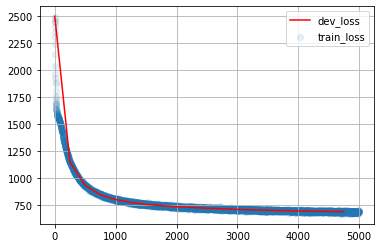
\includegraphics[width=\linewidth]{../catalogue/select-16.png}
  \caption{Visualisation of the training loss of an ML model.}\label{fig:loss}
\end{figure}

\begin{lstlisting}[language=Python, caption={Assertion to check that the mean of the first 10 observations of the loss is higher than the mean of the last 10 observations. In other words, the assertion checks if the loss function is converging to an optimal minima.}, label={lst:loss}]
assert np.mean(train_history[:10], axis=0)[1] > np.mean(train_history[-10:], axis=0)[1], "The model didn't converge."
\end{lstlisting}

In contrast to the assertions presented in Table~\ref{tab:compare-op-asserts}, Listing~\ref{lst:loss} presents an assertion that ensures that the model performs well, without using a magic threshold. The assertion checks if the mean of the first 10 observations of the loss is higher compared to the mean of the last 10 observations. In other words, the assertion ensures that the loss of the model decreased after training, and that the model was able to ``learn'' from the training set. The assertion is derived from the visualisation presented in Figure~\ref{fig:loss}, which shows the loss of the model over the training epochs.

\begin{figure}
  \subcaptionbox{Histogram showing the distribution of a feature before and after scaling.\label{fig:scale}}{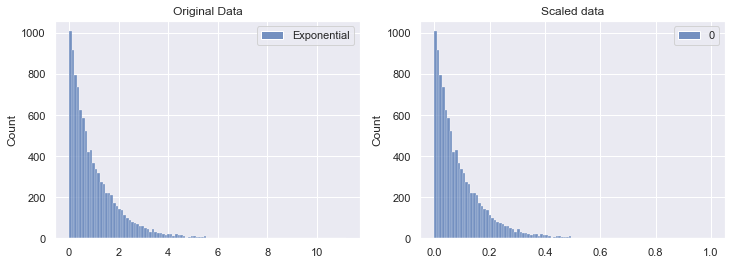
\includegraphics[width=\linewidth]{../catalogue/select-65a.png}}
  \subcaptionbox{Histogram showing the distribution of a feature before and after normalisation.\label{fig:normal}}{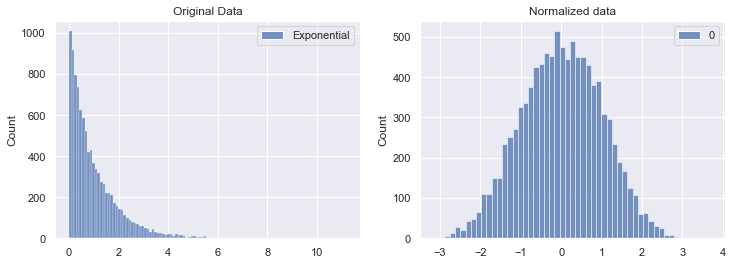
\includegraphics[width=\linewidth]{../catalogue/select-65b.png}}
  \caption{Visualisation of data before and after various data pre-processing techniques.}
  \label{fig:data-pre-process}
\end{figure}

\begin{lstlisting}[language=Python, caption={Assertion to check that the mix and max of a feature fall within specified threshold derived from the visualisation presented in Figure~\ref{fig:scale}.}, label={lst:scale}]
assert scaled_data[scaled_data.argmax()] <= 1
assert scaled_data[scaled_data.argmix()] >= 0
\end{lstlisting}

\begin{lstlisting}[language=Python, caption={Similar premise as Listing~\ref{lst:scale}, however this assertion is based on Figure~\ref{fig:normal}.}, label={lst:normal}]
assert normalized_data[normalized_data.argmax()] < 10
assert normalized_data[normalized_data.argmin()] > -7
\end{lstlisting}

Visualisations in Figure~\ref{fig:data-pre-process} were obtained from a notebook that presents a tutorial on scaling and normalization---two common data pre-processing techniques in ML. The visualisations show a comparison of the data before and after each pre-processing technique is applied to a feature from the dataset. The author performs a visual check, by comparing the distribution of the data before and after applying the pre-processing technique, using a histogram.

Listing~\ref{lst:scale} and~\ref{lst:normal} show the assertions that were defined below Figure~\ref{fig:scale} and~\ref{fig:normal} respectively. Both assertions check that the min and max of the feature is within the expected bounds after applying the respective pre-processing technique. In contrast to assertions presented in Table~\ref{tab:compare-op-asserts}, it is clear that the thresholds are derived from the corresponding visualisations.

\begin{lstlisting}[language=Python, caption={Assertion to check that an augmented image is different from the original.}, label={lst:no-comp-magic}]
assert not np.allclose(x_aug, x_original)
\end{lstlisting}

22\% of the assertions did not use a comparison operator, nor a magic threshold. Listing~\ref{lst:no-comp-magic} highlights such an assertion which is obtained from a notebook that performs image augmentation using Weighted K-Nearest Neighbours. The assertion compares the matrix representation of two images, and checks that the augmented image is different from the original.

Most notebooks examined in this study do not use any external testing libraries. 227 or 84\% of the VA pairs use the low-level Python \texttt{assert} statement to define the test directly. This aligns with our observations that majority of the assertions compare the value of a performance metric against a user defined threshold, and do not require the use of a specialised testing library. 

This study found 42 VA pairs where an external testing library was used. Listing~\ref{lst:np-almost-equal} shows an assertion that uses the \texttt{assert\_almost\_equal} method from the \texttt{numpy.testing} module. The assertion checks if the loss of the model is similar to the specified value, up to a desired precision. Due to the stochastic nature of ML, results obtained from two separate development cycles will slightly differ. The assertion presented in Listing~\ref{lst:np-almost-equal} is found to be robust towards such perturbations and will only fail if there is a significant change in the performance of the model.

\begin{lstlisting}[language=Python, caption={Assertion to check that the loss of the model is similar to the specified value.}, label={lst:np-almost-equal}]
ans4 = compute_loss(X_expanded, y, w)
np.testing.assert_almost_equal(ans4, 0.3042764) 
\end{lstlisting}

\subsubsection{Do the assertions capture all the information obtained from the corresponding visualisation?}
We performed an in-depth analysis of 34 unique VA pairs. This was conducted by reading and understanding the entire contents of the notebooks in a top-down order. During the analysis, several data points such as the primary objective of the notebook, the type of ML problem, the type of ML model and the type of data were captured. We find several instances of VA pairs where the assertion is unable to capture all the information obtained from the visualisation.

\begin{figure}
  \subcaptionbox{Visualisation of the decision boundary of a SVM with a linear kernel.\label{fig:svm-linear}}{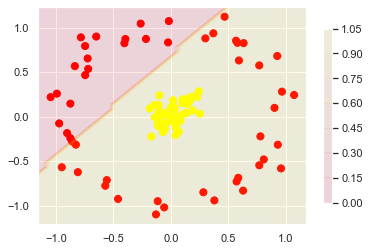
\includegraphics[width=0.49\linewidth]{../catalogue/select-04-linear.png}}
  \hfill
  \subcaptionbox{Visualisation of the decision boundary of a SVM with a RBF kernel.\label{fig:svm-rbf}}{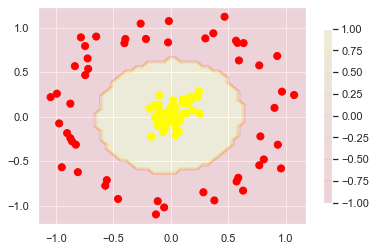
\includegraphics[width=0.49\linewidth]{../catalogue/select-04-rbf.png}}
  \caption{Visualisation of the decision boundary of a SVM trained using different kernels.}\label{fig:svm}
\end{figure}

\begin{lstlisting}[language=Python, caption={Assertion on the accuracy of the ML model.}, label={lst:svm}]
assert accuracy_score(y_test, pred) > 0.95
\end{lstlisting}

Figure~\ref{fig:svm} and Listing~\ref{lst:svm} present one such pair. Visualisations~\ref{fig:svm-linear} and~\ref{fig:svm-rbf} are obtained from a notebook that performs binary classification using Support Vector Machines (SVM). The visualisations show the two classes present in the training set, and the decision boundary of the model when trained first using a linear kernel and later with a RBF kernel.

The visualisations contain several useful information that can be used to test and debug ML models. For instance, using Visualisation~\ref{fig:svm}, ML practitioners can get a visual understanding of how well the model is able to classify the two classes in the dataset. Additionally, observing the complexity of the decision boundary is a quick way to determine if the model is under or overfitting the data. The visualisation also allows comparison of different ML models or variants, to iteratively find a model and hyper-parameters that best fits the underlying training data. In this case for instance, the author of the notebook first trained the SVM with a linear kernel. And upon realising that the data is not linearly separable, chose the RBF kernel.

Listing~\ref{lst:svm} shows the corresponding assertion that was defined below the visualisations. The assertion checks if the model accuracy is above a threshold specified by the author. The assertion however, is only able to capture the information pertaining to the performance of the model. While the rest of the information that is gained from the qualitative assessment using visualisation is lost.

\begin{lstlisting}[language=Python, caption={Assertion to check that the Coefficient of Determination ($R^2$) is higher than the specified threshold.}, label={lst:r2}]
r2_gru = r2_score(y_test, y_pred)
assert r2_gru > 0.6
\end{lstlisting}

\begin{figure}
  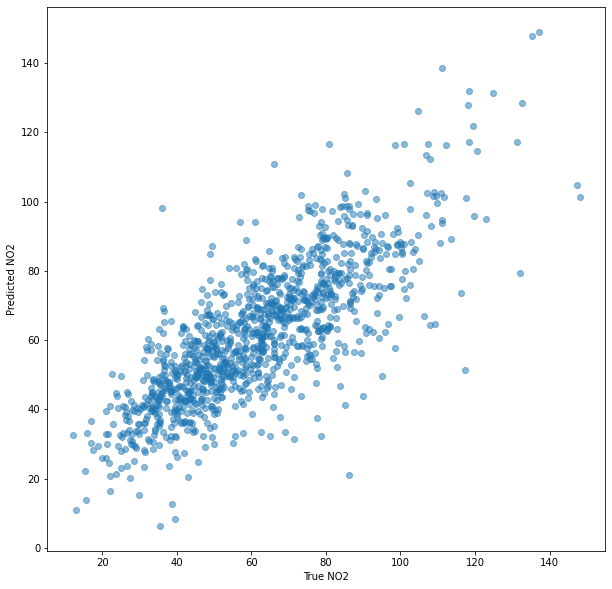
\includegraphics[width=\linewidth]{../catalogue/select-332a.png}
  \caption{Scatter plot of the actual and predicted labels of a dataset. The visualisation shows that there is a linear relationship between the true and predicted labels.}\label{fig:r2}
\end{figure}

Figure~\ref{fig:r2} shows a visualisation obtained from a notebook that trains a RNN to predict the levels of Nitrogen Dioxide ($NO_2$) in the next 24 hour window. The visualisation shows a scatter plot of the real and predicted values of $NO_2$ from the test set. A linear relationship between the ground truth and predictions is observed, indicating that the model was able to learn certain patterns from the training data. The spread of $y_{pred}$ at any given $y_{true}$ is wide. For example, at $y_{true} = 80$, the prediction can range anywhere between 30 and 120. This indicates that the model was not able to fit the training data that well, and can be fine-tuned.

Listing~\ref{lst:r2} presents the corresponding analytical test which was defined below Figure~\ref{fig:r2}. The \texttt{r2\_score} method fits a linear regression model on the true and predicted labels and computes the Coefficient of Determination ($R^2$) based on the residuals of the linear regression model. The assertion checks that the $R^2$ score of the model is always higher than $0.6$. Since the best score possible is $1.0$, the specified threshold indicates that the author wants to ensure that $y_{pred}$ and $y_{true}$ are always linearly related to each other.

Similar to Figure~\ref{fig:svm}, the visualisation in Figure~\ref{fig:r2} allows ML practitioners to visually assess if the model is under or overfitting the training data. If the spread of $y_{pred}$ is wide, it indicates that the model is under-fitting. In contrast, if the spread is very close to the diagonal line, it indicates that the model is most likely overfitting. The visualisation can also be used to verify if there are any outliers in the predictions, for a given input. The assertion in Listing~\ref{lst:r2} however, does not capture such information. It can only check if the performance of the model is better than a specific threshold.

\begin{lstlisting}[language=Python, caption={Assertion to check that each feature in a dataset is normal using the Kolmogorov-Smirnov test for goodness of fit from the scipy library.}, label={lst:kstest}]
for feature in range(data_transformed.shape[1]):
  assert kstest(data_transformed[:, feature], 'norm').statistic < 1e-2
\end{lstlisting}

\begin{figure}
  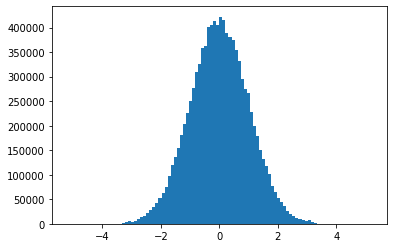
\includegraphics[width=\linewidth]{../catalogue/select-152a.png}
  \caption{Visualisation of the distribution of a feature from the dataset.}\label{fig:kstest}
\end{figure}

In contrast to Listing~\ref{lst:svm} and Listing~\ref{lst:r2}, Figure~\ref{fig:kstest} and Listing~\ref{lst:kstest} present a VA pair where the assertion captures all the information obtained from the visualisation.

The notebook author normalises the training data and performs a visual check using the visualisation presented in Figure~\ref{fig:kstest}. The visualisation shows a bell-shaped curve thus indicating that the data is normal and that the transformation was successful. The assertion in Listing~\ref{lst:kstest} formally verifies that all features in the dataset have a normal distribution. The assertion iterates through each column in the dataset and performs the Kolmogorov-Smirnov test to check that the distribution of the feature is similar to that of a normal distribution.

Checking the distribution of the training data is a very common task performed during the data understanding or exploratory data analysis phase of the ML development lifecycle. Several ML models assume normality in the underlying training data. However, in a production environment where ML models are continually trained using new batches of data, this assumption of normality may not always hold. The formal assertion presented in Listing~\ref{lst:kstest} makes this assumption explicit. And causes the automated ML pipeline to fail if our expectations regarding the data are no longer satisfied.

\section{Implications}\label{sec:discuss}
% NOTE: from ICST paper, need to integrate...

% NOTE: breck2017ml proposes feature and data testing; we can say that the assertions in the notebook bring the system closer to migrating them into dedicated data validation systems 

% NOTE: perhaps also argue the other side, the demographic using notebooks do not have SE training; they are perhaps directly sharing the notebook and the data directly...
P71 highlights the lack of proper software engineering best practices within Jupyter notebooks. This shortcoming in computational notebooks has been identified by prior studies~\cite{quaranta2021kgtorrent, pimentel2019large-scale}. In this case study, managing dependencies through external tools is recommended. Python's built-in \emph{requirements.txt}~\footnote{https://pip.pypa.io/en/stable/reference/requirements-file-format/} file allows specifying dependencies and versions. Alternatively, external programs like \emph{pipenv}~\footnote{https://pipenv.pypa.io/en/latest/} and \emph{poetry}~\footnote{https://python-poetry.org/} use lockfiles to ensure specific version control, guaranteeing reproducibility across different systems. 

% NOTE: think about the actors: educators, researchers, developers...
The results from RQ1 provide empirical evidence to support the use of
visualisations to test various properties of ML systems.
Visualisations are an efficient and effective medium to present
complex information, that is easier to interpret by humans with the
aid of visual cues. Visualisations used to test ML system properties
however, demand manual verification effort. Information gained from
visualisations and subsequent decisions made based on this
information, must be manually verified in every iteration of the ML
development cycle.

% NOTE link to accumulation of technical debt due to highly
% experimental nature, and constant change in the system

Assertions or analytical tests extracted from ML visualisations can
reduce this manual verification effort. Assertions encapsulate the
knowledge gained from the visualisation with regards to the property
of the ML system which is currently under test. Formal assertions
document the observations made by the AI practitioner regarding the
model or the data, at a specific point in time. These observations
should not be violated by the future model development cycles unless
the requirements of the ML system are changed. Assertions scale across
organisational or personnel changes as future AI practitioners can
refer to the assertions to understand how the visualisations were
previously interpreted.

The results for RQ1 indicate that the combination of ML visualisations
with analytical assertions is an emerging testing practice within the
machine learning community. We found only $54,070$ notebooks that
contain the keyword ``assert'', while there are more than a million
Jupyter notebooks available on GitHub. This suggests that writing
assertions in computational notebooks is still relatively uncommon. We
believe that this is due to a lack of knowledge among practitioners
regarding testing approaches and the absence of adequate tooling to
support the assertion of model properties. We argue that guidelines on
ML coding practices require improvement. And advocate the need to
steer education and research of Software Engineering practices towards
the specific challenges faced when contributing to ML software
systems.

In the 1764 notebooks analysed in this study, several visualisations
lack assertions. However, implicit expectations still exist within
each visualisation which cannot be readily validated by other project
collaborators. ML testing demands proficiency in Machine Learning,
Software Testing, and the underlying Mathematical concepts. This
further highlights the need for refining the education for these
professionals and crafting tools to compensate for gaps in their
knowledge.

Results from RQ2 reveal two challenges in the current landscape of ML
testing. The assertions in the VA pairs identified in this study lack
dedicated testing libraries. This indicates that the current culture
of testing ML code is still in its infancy and ML practitioners are
not yet exploring software testing libraries. Second, the existing
testing libraries are not tuned to the specifics of ML code and
practitioners have to fall back to basic built-in approaches.

The widespread use of ``magic'' thresholds---often rooted in domain
expertise or experience obtained over time---poses risks to
maintainability of ML projects. We advocate that such thresholds are
documented for future reference. And find a clear need for automated
tools that highlight undocumented choices or suggest standardized
documentation in Markdown or code annotations.

In the results from RQ3, we see several examples of assertions that
fail to capture all the information gained from its visual
counter-part. This can lead to a mismatch of expectations in future
versions of the ML software. For instance, another project
collaborator might run the code with a new version of the dataset or a
different learning technique and assume that if the assertions run
successfully, the expected patterns from the visualisation are also
satisfied. The examples presented in Section~\ref{sec:result-rq3} show
that deriving assertions from visualisations is not trivial. Basic
visualisation patterns require complex mathematical techniques which
may be beyond the expertise of an ML developer.

For example, a linear correlation between the true and predicted
labels is evident in Figure~\ref{fig:r2}. Yet, its formal assertion in
Listing~\ref{lst:r2} necessitates defining an appropriate threshold
for the coefficient of determination metric. Our results show that
current software testing practices fail to capture the idiosyncrasies
of ML code. There is a pressing need for automated tools, that bridge
the disparity between the qualitative evaluation of ML systems using
visualisations and the extraction of analytical assertions from these
visuals.


% BibTeX users please use one of
% \bibliographystyle{spbasic}      % basic style, author-year citations
\bibliographystyle{spmpsci}      % mathematics and physical sciences
%\bibliographystyle{spphys}       % APS-like style for physics
\bibliography{bibliography}   % name your BibTeX data base

\end{document}
% end of file template.tex

